%%%%%%%%%%%%%%%%%%%%%%%%%%%%%%%%%%%%%%%%%%%%%%%%%%%
%
%  New template code for TAMU Theses and Dissertations starting Fall 2016.
%
%  Author: Sean Zachary Roberson
%	 Version 3.16.09
%  Last updated 9/12/2016
%
%%%%%%%%%%%%%%%%%%%%%%%%%%%%%%%%%%%%%%%%%%%%%%%%%%%

%%%%%%%%%%%%%%%%%%%%%%%%%%%%%%%%%%%%%%%%%%%%%%%%%%%%%%%%%%%%%%%%%%%%%%%
%%%                           SECTION II
%%%%%%%%%%%%%%%%%%%%%%%%%%%%%%%%%%%%%%%%%%%%%%%%%%%%%%%%%%%%%%%%%%%%%%


\chapter{Improved Quasi-Static Method}
%%%%%%%%%%%%%%%%%%%%%%%%%%%%%%%%%%%%%%%%%%%%%%%%
\section{Theory}
\label{sect:theory}
%%%%%%%%%%%%%%%%%%%%%%%%%%%%%%%%%%%%%%%%%%%%%%%%

To derive the IQS equations, the time dependent neutron diffusion equation with delayed neutron precursors are presented by Equations~\ref{eq:flux}~and~\ref{eq:precursor}.

\begin{subequations}
\begin{multline}
\frac{1}{v^g}\frac{\partial \phi^g}{\partial t}  = 
\frac{\chi_p^g}{\keff} (1-\beta)\sum_{g'=1}^G  \nu^{g'} \Sigma_f^{g'} \phi^{g'} 
+ \sum_{g'\neq g}^G\Sigma_s^{g'\to g} \phi^{g'}  \\ + \sum_{i=1}^I\chi_{d,i}^g\lambda_i C_i 
-  \left( -\div D^g \grad  + \Sigma_r^g \right) \phi^g   
\ , \quad 1 \le g \le G 
\label{eq:flux}
\end{multline}
\be
\frac{dC_i}{dt} = \frac{\beta_i}{\keff}\sum_{g=1}^G\nu^{g} \Sigma_f^g \phi^{g} - \lambda_i C_i \ , \quad 1 \le i \le I 
\label{eq:precursor}
\ee
\end{subequations}

where,

\begin{longtable}{lll}
$\phi^g$   			&	$=$	&	Scalar flux in energy group $g$ \\
$C_i$					  &	$=$	&	Concentration of delayed neutron precursor $i$ \\
$\Sigma_f^{g}$	&	$=$	&	Fission cross section in energy group $g$ \\
$\Sigma_r^{g}$	&	$=$	&	Removal cross section in energy group $g$ \\
$\Sigma_s^{g' \to g}$	&	$=$	&	Scattering cross section from energy group $g'$ to $g$ \\
$v^g$					  &	$=$	&	Neutron velocity in energy group $g$ \\
$\chi_p^g$			&	$=$	&	Fission spectrum of prompt neutrons \\
$\chi_{d,i}^g$	&	$=$	&	Fission spectrum of delayed neutrons from precursor $i$ \\
$\nu^g$					&	$=$	&	Total number of neutrons per fission \\
$D^g$					  &	$=$	&	Diffusion coefficient in energy group $g$\\
$\lambda_i$			&	$=$	&	Decay constant of precursor $i$ \\
$\beta_i$				&	$=$	&	Delayed neutron fraction  from precursor $i$ \\
$\beta$			 	  &	$=$	&	Total delayed neutron fraction ($\beta = \sum_{i=1}^I \beta_{i}$) \\
  & & 
\end{longtable}

Most reactor computation frameworks, including Rattlesnake, discretize the time variable directly with these equations using a multitude of schemes (Implicit Euler, Crank-Nicholson, implicit Runge-Kutta, etc.).  In this paper, the method of discretizing Equations~\ref{eq:flux}~and~\ref{eq:precursor} is generally referred to as ``implicit discretization''.  This research intends to improve upon this method by instead implementing the improved quasi-static method (IQS) for neutron kinetics and
implement it within a multiphysics setting.

IQS involves factorizing the flux from \eqt{eq:flux} into time-dependent amplitude ($p$) and space- and time- dependent shape ($\varphi$).  The resulting equation is the shape-diffusion equation with precursors represented by Equations~\ref{eq:shape}~and~\ref{eq:prec}.

\begin{subequations}
\begin{align}
\frac{1}{v^g}\frac{\partial \varphi^g}{\partial t} = &\frac{\chi_p^g}{\keff} (1-\beta)\sum_{g'=1}^G  \nu^{g'} \Sigma_f^{g'} \varphi^{g'} + \sum_{g'\neq g}^G\Sigma_s^{g'\to g} \varphi^{g'} \nonumber \\ 
& -  \left( -\div D^g \grad  + \Sigma_r^g + \boxed{\frac{1}{v^g}\frac{1}{p}\frac{dp}{dt}}\right) \varphi^g + \boxed{\frac{1}{p}}\sum_{i=1}^I\chi_{d,i}^g\lambda_iC_i  , \quad 1 \le g \le G 
\label{eq:shape}
\end{align}
\be
\frac{dC_i}{dt} = \frac{\beta_i}{\keff}\boxed{p} \sum_{g=1}^G\nu^{g} \Sigma_f^g \varphi^{g} - \lambda_i C_i \ , \quad 1 \le i \le I 
\label{eq:prec}
\ee
\end{subequations}

We note that the time-dependent shape equation is similar to the time-dependent flux equation, with the following modifications:
\begin{enumerate}
\item The shape equation contains an additional term equivalent to a removal cross section,  $ \frac{1}{v^g}\frac{1}{p}\frac{dp}{dt}$.
\item The delayed neutron source term is divided by $p$.
\item The system of equations is now nonlinear due to the factorization.
\item An equation is needed to obtain the amplitude $p$.
\end{enumerate}

To derive the amplitude equation, the shape/precursors equations are weighted by a space-dependent function and integrated over the phase-space. The weight function is typically the adjoint flux $\phi^{*g}$, which can be proven to minimize truncation error \cite{duderstadt1976nuclear}. The final expressions are given below:
\begin{subequations}
\be
\frac{dp}{dt}=\left[\frac{\rho-\bar{\beta}}{\Lambda}\right]p+\sum_{i=1}^I\bar{\lambda}_i\xi_i
\label{eq:p}
\ee
\be
\frac{d\xi_i}{dt}=\frac{\bar{\beta}_i}{\Lambda}-\bar{\lambda}_i\xi_i \quad 1 \le i \le I 
\label{eq:c}
\ee
\end{subequations}
This equation is also known as the point reactor kinetics equation (PRKE); where the reactivity, effective delayed-neutron fraction, and delayed-neutron precursor decay constant are defined as follows:
\begin{subequations}
\be
\frac{\rho-\bar{\beta}}{\Lambda} = 
\frac{ \sum_{g=1}^G\left(\phi^{*g},\frac{\chi_p^g}{\keff}(1-\beta)\sum_{g'=1}^G \nu^{g'} \Sigma_f^{g'}\varphi^{g'} + \sum_{g'\neq g}^G\Sigma_s^{g'\to g} \varphi^{g'} -\left( -\div D^g \grad  + \Sigma_r^g \right)\varphi^g\right)}
{\sum_{g=1}^G\left(\phi^{*g},\frac{1}{v^g}\varphi^g\right)}
\label{eq:rmb}
\ee
\be
\frac{\bar{\beta}}{\Lambda} = \sum_{i=1}^I\frac{\bar{\beta}_i}{\Lambda} = 
\sum_{i=1}^I\frac{1}{\keff}\frac{\sum_{g=1}^G(\phi^{*g}, \chi_{d,i}^g\beta_i\sum_{g'=1}^G\nu^{g'} \Sigma_f^{g' }\varphi^{g'})}
{\sum_{g=1}^G\left(\phi^{*g},\frac{1}{v^g}\varphi^g\right)}
\label{eq:b}
\ee
\be
\bar{\lambda}_i = \frac{\sum_{g=1}^G(\phi^{*g},\chi_{d,i}^g\lambda_i C_i)}{\sum_{g=1}^G(\phi^{*g},\chi_{d,i}^gC_i)}
\label{eq:l}
\ee 
\end{subequations}
The following inner product definition has been used: $\left(\phi^{*g},f\right):=\int_D\phi^{*g}(\vec{r})f(\vec{r})d^3r$.\\  

Additionally, in order to impose uniqueness on the factorization and to derive the PRKE, the following normalization condition is imposed: $\sum_{g=1}^G\left(\phi^{*g},\frac{1}{v^g}\varphi^g\right) = \textit{constant}$ \cite{Dulla2008}. \\

Solving for the shape in \eqt{eq:shape} can become expensive, especially in two or three dimensions, and even more so when using the transport equations in lieu of the diffusion equations.  Using IQS, one expects the time dependence of the shape to be weaker than that of the flux itself,  thus allowing for larger time step sizes in updating the shape. The PRKE equations form a small ODE system and can be solved using a much smaller time step size. In transients where the shape varies much less than the flux, IQS can thus be very computationally effective. The two-time scale solution process, a micro scale for the PRKE and a macro scale for the shape, is illustrated in \fig{fig:iqsviz}.  

\begin{figure}[!htbp]
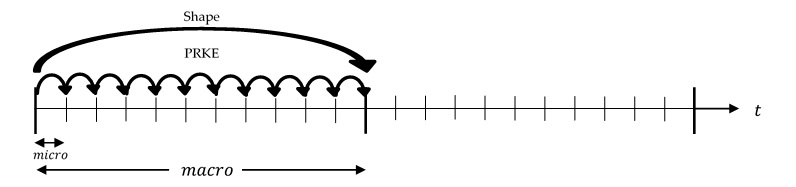
\includegraphics[width=\linewidth]{\FiguresDir/IQS_visualization.jpg}
\caption{IQS method visualization}
\label{fig:iqsviz}
\end{figure}

%%%%%%%%%%%%%%%%%%%%%%%%%%%%%%%%%%%%%%%%%%%%%%%%
\subsection{Operator Notation and Extension of IQS to Multigroup Transport Equations}
\label{sect:transport}

For simplicity, the previous section only described the IQS implementation using the neutron diffusion equation. However, deriving the IQS form for other neutron balance equations (e.g., transport, simplified transport, etc.) is very similar. To this end, we re-write the neutron conservation equations in operator form, shown in \eqt{eq:transport}. 
\be
\frac{\partial}{\partial t}\left(\frac{\Psi^g}{v^g}\right) = \sum_{g'} \left(H^{g'\to g} + P_p^{g' \to g} \right) \Psi^{g'} - L^g\Psi^g + S_d^g
\label{eq:transport}
\ee
where $\Psi^g$ is the multigroup neutron flux (angular flux in the case of transport), $H^{g'\to g}$ is the scattering operator, $P_p^{g' \to g}$ is the prompt neutron production operator, $L^g$ is the loss operator, and $S_d^g$ is the delayed neutron source operator. Using \eqt{eq:flux}, the reader may easily obtain the functional form for these operators in the case of a diffusion approximation.
%
%Factorization is defined as $\Psi^g(\vec{r},\vec{\Omega},t)=p(t)\psi^g(\vec{r},\vec{\Omega},t)$ and the resulting shape equation is defined by \eqt{eq:tshape}.  
Next, the factorization $\Psi^g(\vec{r},\vec{\Omega},t)=p(t)\psi^g(\vec{r},\vec{\Omega},t)$ is introduced, where the shape is denoted by $\psi^g$, leading to the following shape equations, \eqt{eq:tshape}:
\be
\frac{\partial}{\partial t}\left(\frac{\psi^g}{v^g}\right) = \sum_{g'} \left(H^{g' \to g} + P_p^{g' \to g}\right) \psi^{g'} - \left( L^g + \frac{1}{v^g}\frac{1}{p}\frac{dp}{dt}\right) \psi^g + \frac{1}{p} S_d^g
\label{eq:tshape}
\ee
Finally, the PRKE parameters are defined by Equations~\ref{eq:trmb}~and~\ref{eq:tb}, where 
$\left(\Psi^{*g},f^g\right) =$\\ $ \int_{4\pi}\int_D \Psi^{*g}(\vec{r},\vec{\Omega})f^g(\vec{r},\vec{\Omega})d^3r d^2\Omega$.
\be
\frac{\rho-\bar{\beta}}{\Lambda}=\frac{ \sum_{g=1}^G\left(\Psi^{*g},\sum_{g'}(H^{g' \to g}g+P_p^{g' \to g}-L^{g'}\delta_{g'g})\psi^{g'}\right)}{\sum_{g=1}^G\left(\Psi^{*g},\frac{1}{v^g}\psi^g\right)}
\label{eq:trmb}
\ee
\be
\frac{\bar{\beta}}{\Lambda}=\sum_{i=1}^I\frac{\bar{\beta}_i}{\Lambda}=\sum_{i=1}^I\frac{\sum_{g=1}^G(\Psi^{*g}, \sum_{g'} P_{d,i}^{g' \to g} \psi^{g'})}{\sum_{g=1}^G\left(\Psi^{*g},\frac{1}{v^g}\psi^g\right)}
\label{eq:tb}
\ee
where $P_{d,i}^{g' \to g}$ is the delayed-neutron operator for precursor group $i$. \\
\indent This section is simply meant to show the theoretical expandability of IQS to transport problems and its derivation in operator notation.  As stated previously, this research only applies and tests IQS with diffusion problems.

%%%%%%%%%%%%%%%%%%%%%%%%%%%%%%%%%%%%%%%%%%%%%%%%
\section{Iterative Solution Techniques}
\label{sect:iter}
%%%%%%%%%%%%%%%%%%%%%%%%%%%%%%%%%%%%%%%%%%%%%%%%

As we noted in \sct{sect:theory}, shape-PRKE equations are a nonlinear system and thus may be solved in a iterative manner.  Each macro time step can be iterated so the best shape is used to compute power at the micro time steps. Sissaoui et al. from \cite{Sissaoui_1995}, Koclas et al. from \cite{Koclas_1996}, Devooght et al. from \cite{Devooght_1984}, and Monier from \cite{Monier_diss} all use iterative techniques for their quasi-static simulations.  They all undergo a similar process:
\begin{itemize}
\item[\textit{Step 1:}] Compute the PRKE parameters at the end of the macro step using the last computed shape
\item[\textit{Step 2:}] Linearly interpolate the computed PRKE parameters over the macro step
\item[\textit{Step 3:}] Solve the PRKE on micro steps over the entire macro step
\item[\textit{Step 4:}] Solve the shape equation on the macro step using the computed values of $p$ and $dp/dt$.
\item[\textit{Step 5:}] Check if the shape solution has converged:
	\begin{itemize}
	\item \textit{No:} Repeat the same macro time step
	\item \textit{Yes:} Move on to the next macro time step
	\end{itemize}
\end{itemize}
This process can be visualized by \fig{fig:picard}.
\begin{figure}[!htpb]
\centering
\begin{tikzpicture}[every node/.style = {font=\normalsize}]

\node[greenblock](p1) at (0,0) {Solve shape equations \\ over macro time step};
\node[greenblock](p2) at (0,-2.5) {Compute PRKE parameters \\ over macro time step};
\node[greenblock](p3) at (0,-5) {Solve PRKE using micro \\ steps};
\node[greenblock](p4) at (0,-7.5) {Update $p$ and $\frac{dp}{dt}$};
\node[blueblock2] (p5) at (0,-11) {Solve other physics \\ components};
\node[reddiamond] (check) at (0,-15) {Check for \\ convergence};
\node [above =0.1mm of p1] {\large{IQS Solve:}};
\node [above =0.1mm of p5] {\large{Multi-physics:}};

\tikzback{p1}{p1}{p4}{p4}{bk1}
\tikzback{p5}{p5}{p5}{p5}{bk2}

\draw[->,ultra thick](p1.south) -- (p2.north);
\draw[->,ultra thick](p2.south) -- (p3.north);
\draw[->,ultra thick](p3.south) -- (p4.north);
\draw [->,ultra thick] (p4.south)+(0,-0.25) -- node [above] {} (bk2-n);
\draw[->,ultra thick](p5.south)+(0,-0.25) -- (check.north);
%\draw[->,ultra thick](check.west) -- (-5,-15) -- node[above,sloped] {\large{no}}(-5,0) -- node[above] {}(bk1-w);
\draw[->,ultra thick](check.west) -- node[above,sloped] {\large{no}} (-5,-15) |-  node[above] {}(bk1-w);
\draw[->,ultra thick](check.south) -- node[right] {\large{yes}} ++(0,-2);

\end{tikzpicture}
\caption{Visualization of IQS fixed-point iteration process}
\label{fig:picard}
\end{figure}

The major difference between the methods of these authors is the convergence criteria used.  Sissaoui and Koclas \cite{Sissaoui_1995, Koclas_1996} use fixed point iteration where the criteria is the simply the normalized difference between the last two computed shapes.  Monier in \cite{Monier_diss} also does fixed point iterations with the same criteria, except the solution is scaled by $\frac{\sum_{g=1}^G\left(\phi^{*g},\frac{1}{v^g}\varphi^g(t_{n})\right)}{\sum_{g=1}^G\left(\phi^{*g},\frac{1}{v^g}\varphi^g(t_{n+1})\right)}$ after each iteration.  Devooght in \cite{Devooght_1984} does a Newton-SOR iteration where the residual of the shape function evaluation is the convergence criteria and next iteration's solution is computed using Newton-Raphson method.\\

These techniques are by no means an exhaustive list of the possible iteration techniques for IQS. Dulla et al. in \cite{Dulla2008} does an in depth analysis of the fixed point iteration technique most similar to Sissaoui and Koclas, involving convergence rates and solution results.  However, no comprehensive analysis of iteration techniques exists, comparing both Newton and fixed-point convergence rates.  The following sections describes each iteration technique investigated by this research.

%%%%%%%%%%%%%%%%%%%%%%%%%%%%%%%%%%%%%%%%%%%%%%%%
\subsection{Shape Convergence}

The most obvious convergence criteria is to observe the change in the shape from one iteration to the next.  Monier in \cite{Monier_diss} observes the $L^{\infty}$ norm of the shape for the convergence criteria, described in \eqt{eq:shape_Linf}.  However, any norm can be used for the criteria, so a $L^2$ norm is another possible criteria, described by \eqt{eq:shape_L2}.
\be
\frac{\text{max}\left|\varphi_{n}^{(k+1)} - \varphi_{n}^{(k)}\right|}{\text{max}\left|\varphi_{n}^{(k+1)}\right|} < \epsilon_{\varphi}
\label{eq:shape_Linf}
\ee 
\be
\frac{\norm{\varphi_{n}^{(k+1)} - \varphi_{n}^{(k)}}}{\norm{\varphi_{n}^{(k+1)}}} < \epsilon_{\varphi}
\label{eq:shape_L2}
\ee 

Where $n$ is the time step, $k$ is the iteration number, and $\epsilon_{\varphi}$ is the numerical criteria provided by a user.  There is no guarantee that the shape converges, so max number of iterations is typically enforced.


%%%%%%%%%%%%%%%%%%%%%%%%%%%%%%%%%%%%%%%%%%%%%%%%
\subsection{Property Convergence}

Monier in \cite{Monier_diss} describes other properties, other than shape, to observe for convergence, shown in Equations \eqref{eq:rho_conv} - \eqref{eq:K_conv}.  These criteria can be added constraints to \eqt{eq:shape_Linf} or be in supplement to.
\be
\left(\frac{\rho}{\Lambda}\right)^{(k+1)} - \left(\frac{\rho}{\Lambda}\right)^{(k)} < \epsilon_{\rho}
\label{eq:rho_conv}
\ee
\be 
p_n^{k+1} - p_n^{k} < \epsilon_p
\label{eq:p_conv}
\ee
\be 
\frac{K_n^{(k+1)} - K_0}{K_0} < \epsilon_K
\label{eq:K_conv}
\ee

Where $K$ is the IQS uniqueness expression:
\be 
K_n^{(k+1)} = \sum_{g=1}^G\left(\phi^{*g},\frac{1}{v^g}\varphi_n^{g,(k+1)}\right)
\label{eq:K}
\ee

$\epsilon_{\rho}$ is the reactivity convergence criteria, $\epsilon_{p}$ is the amplitude convergence criteria, and $\epsilon_{K}$ is the constraint convergence criteria.

%%%%%%%%%%%%%%%%%%%%%%%%%%%%%%%%%%%%%%%%%%%%%%%%
\subsection{Solution Scaling}

In order to preserve the uniqueness criteria, it is beneficial to scale the shape such that the $K_n$ is constant, shown in \eqt{eq:shape_scale}.  This scaling can also be done after each iteration, to insure that the uniqueness criteria is satisfied whenever the shape is evaluated.
\be 
\varphi^{g}_n = \varphi^{g,(\text{last})}_n \frac{K_0}{K^{(\text{last})}_{n}}
\label{eq:shape_scale}
\ee

%%%%%%%%%%%%%%%%%%%%%%%%%%%%%%%%%%%%%%%%%%%%%%%%
\subsection{Preconditioned Jacobian-Free Newton-Krylov}

By far, the most common nonlinear system iteration method in MOOSE is Preconditioned Jacobian-Free Newton-Krylov with Generalized Minimal RESidual method (GMRES) as the linear system solver.  This section only descirbes the methods' application to IQS; a very detailed description of PJFNK is transcribed by Knoll in \cite{PJFNK_Knoll}. Essentially, the IQS system of equations can be described by \eqt{eq:IQSsys}.  Where $A$ is a matrix operator, $\varphi$ is the solution vector, and $F$ is the forcing vector.
\be
A(\varphi(p))\varphi=F(\varphi,p,t)
\label{eq:IQSsys}
\ee
Applying the residual based Newton-method yields:
\be
J\delta\varphi = -R(\varphi,p)
\ee 
Where $J$ is the Jacobian matrix defined as $J_{ij}=\partial R_i/\partial\varphi_j$, $\delta\varphi$ is the error in the iterating solution, and $R$ is the residual vector defined as $A\varphi-F$ (most methods simply define the residual instead of evaluating this expression).  For IQS, a residual evaluation entails a PRKE parameter evaluation and the PRKE evaluation over the entire macro-step.  Applying a preconditioner $P$ yields:
\be 
(JP^{-1})(P\delta\varphi)=-R(\varphi,p)
\ee
This resulting system can be split into two systems, represented by Equations~\eqref{eq:PJFNK_1}~and~\eqref{eq:PJFNK_2}.
\be 
(JP^{-1})w = -R(\varphi,p)
\label{eq:PJFNK_1}
\ee
\be 
\delta\varphi = P^{-1}w
\label{eq:PJFNK_2}
\ee
Solving \eqt{eq:PJFNK_1} requires the evaluation of Jacobian operator, which is done each GMRES iteration in two steps:
\begin{enumerate}
\item Approximately solve the preconditioner system for $y$: $Py=w$
\item Perform matrix-free Jacobian operation: $Jy\approx[R(\varphi+\epsilon y,p')-R(\varphi,p)]/\epsilon$
\end{enumerate}
This Jacobian operation is a finite difference approach.  $\epsilon$ is a perturbation scalar and $p'$ is the amplitude computed with PRKE parameters calculated from the perturbed shape.  For IQS, the PRKE and its parameters must be evaluated for the perturbed and original system, although the unperturbed residual is stored from the beginning of the PJFNK iteration.

%%%%%%%%%%%%%%%%%%%%%%%%%%%%%%%%%%%%%%%%%%%%%%%%
\section{Predictor-Corrector version of IQS (IQS P-C)}
\label{sect:pc}
%%%%%%%%%%%%%%%%%%%%%%%%%%%%%%%%%%%%%%%%%%%%%%%%

The Predictor-Corrector (P-C) version of IQS factorizes the flux and derives the PRKE the same way as the standard version, but the solution of the coupled system of equations is different.  In the IQS P-C version, the flux equations (not the shape equations) are solved (represented by Equations~\ref{eq:flux}~and~\ref{eq:precursor}) in order to obtain a predicted flux solution. This predicted flux is then converted to a shape by rescaling it as follows:
\be
\varphi^g_{n+1} = \underbrace{\phi^g_{n+1}}_{\text{predicted}} \frac{K_0}{K_{n+1}}
\label{eq:rescale}
\ee
where the scaling factors are given by
\be
K_{n+1} =\sum_{g=1}^G\left(\phi^{*g},\frac{1}{v^g}\phi^g_{n+1}\right)
\ee
\be
K_{0} =\sum_{g=1}^G\left(\phi^{*g},\frac{1}{v^g}\varphi^g_{n+1}\right)=\sum_{g=1}^G\left(\phi^{*g},\frac{1}{v^g}\phi^g_{0}\right)
\ee

The PRKE parameters are then computed with this shape using Equations~\ref{eq:rmb}~-~\ref{eq:l} and interpolated over the macro step, then the PRKE ODE system is solved on the micro time scale.  With the newly computed amplitude, the shape is rescaled into a flux and the final corrected flux is given by:
\be
\underbrace{\phi^g_{n+1}}_{\text{corrected}} = p_{n+1} \times \varphi^g_{n+1} \,.
\ee

The advantage to the predictor-corrector method is there is no iteration necessary for this method and, in turn, is much simpler and faster than the standard IQS.  Ikeda et al. in \cite{Ikeda_2001} and Goluoglu et al. in \cite{Goluoglu_2001} both use IQS P-C for complex, three-dimensional problems.  Their results prove IQS P-C to be impressively effective, despite the de-coupling of the system.  Dulla et al. in \cite{Dulla2008} also describes an in depth comparison of IQS P-C with traditional IQS.


%%%%%%%%%%%%%%%%%%%%%%%%%%%%%%%%%%%%%%%%%%%%%%%%
\section{Temperature Feedback}
\label{sect:mp}
%%%%%%%%%%%%%%%%%%%%%%%%%%%%%%%%%%%%%%%%%%%%%%%%

IQS is first and foremost a nuclear reactor simulation method.  In nuclear reactors, multiple physics affect the profile of the neutron flux.  The most simple example of mulitphysics reactor simulations is adiabatic heat up with Doppler feedback. The principle of Doppler feedback is that fission in a fuel causes the material to increase temperature and induces a change in the neutronics properties.  The material heat up is described by \eqt{eq:temp}; where $\rho$ is the material density, $c_p$ is the specific heat, $T$ is temperature, and $\kappa_f$ is the energy released per fission \cite{ANL_BPB}. The change in temperature of the material mainly affects the thermal macroscopic absorption cross section described by \eqt{eq:dopp} \cite{ANL_BPB}.

\be
\rho c_p \frac{\partial T(\vec{r},t)}{\partial t} = \kappa_f \sum^G_{g=1}\Sigma_f^g \phi^g(\vec{r},t)
\label{eq:temp}
\ee

\be
\Sigma_a^{thermal}(\vec{r},t) = \Sigma_a^{thermal}(\vec{r},0)\left[1+\gamma\left(\sqrt{T}-\sqrt{T_0}\right)\right]
\label{eq:dopp}
\ee

%%%%%%%%%%%%%%%%%%%%%%%%%%%%%%%%%%%%%%%%%%%%%%%%
\subsection{Temperature Evaluation}

Temperature evaluation (\eqt{eq:temp}) is quite similar to the evaluation of the delayed neutron precursors from \sct{sect:dnp}. A typical implicit solver would simply use the interpolated flux at end of the temperature time step for the right hand side of the equation, a theta-method discretization.  However, IQS has much more information about the profile of the flux along the time step because of the micro-step amplitude evaluation.  Therefore, it is possible to solve for temperature using a semi-analytical approach, shown by \eqt{eq:temp_an}.
\be
T^{n+1} = T^n + \frac{\kappa_f}{\rho c_p} \left(a_2 \varphi^{n+1} + a_1 \varphi^{n}\right)
\label{eq:temp_an}
\ee
Where $n$ corresponds to the beginning of the temperature step.  $a_1$ and $a_2$ are integration coefficients defined by \eqt{eq:a1} and \eqt{eq:a2}.  Any interpolation of the amplitude along the micro steps is possible for the integration, this application uses piece-wise linear.
\be
a_1 = \int_{t_n}^{t_{n+1}}\left(\frac{t_{n+1}-t'}{\Delta t}\right)p(t')dt'
\label{eq:a1}
\ee
\be
a_2 = \int_{t_n}^{t_{n+1}}\left(\frac{t'-t_n}{\Delta t}\right)p(t')dt'
\label{eq:a2}
\ee

%%%%%%%%%%%%%%%%%%%%%%%%%%%%%%%%%%%%%%%%%%%%%%%%
\subsection{Intermediate Time Scale}

For IQS, this temperature feedback affects both the shape equation and the reactivity of the PRKE; thus, it is an additional nonlinear component to the already coupled shape-amplitude equations. In foresight to the application of this component, temperature is much more time dependent than the shape, but less so than the amplitude.  Therefore, the evaluation of temperature will have its own time scale.  A possible solution process for a problem with temperature feedback will have time three time scales portrayed in \fig{fig:time}.  The first time scale is the shape solve, the second is the temperature evaluation as well as the computation of PRKE parameters, and the third is the PRKE scale.  It is important to note that the number of time steps in each scale is arbitrary and meant only for visual purposes.

\begin{figure}[htpb!]
\centering
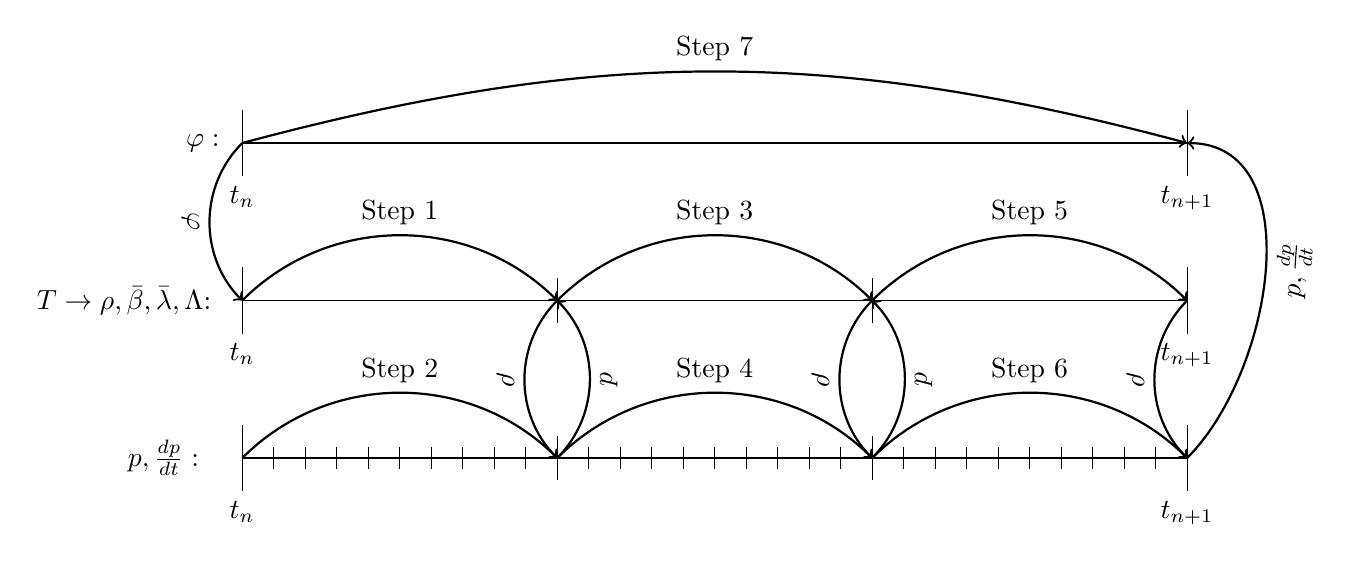
\begin{tikzpicture}[scale=2]
%Shape
\draw[] (0,2) -- (6,2) ;
\foreach \x in  {0,6}
\draw[shift={(\x,2)},color=black] (0pt,6pt) -- (0pt,-6pt);
\draw[shift={(0,2)},color=black] (0pt,0pt) -- (0pt,-6pt) node[below] {$t_n$};
\draw[shift={(6,2)},color=black] (0pt,0pt) -- (0pt,-6pt) node[below] {$t_{n+1}$};
\node(shape) at (-.25,2) {$\varphi:$};

%Temp/Params
\draw[] (0,1) -- (6,1) ;
\foreach \x in  {0,6}
\draw[shift={(\x,1)},color=black] (0pt,6pt) -- (0pt,-6pt);
\foreach \x in  {2,4}
\draw[shift={(\x,1)},color=black] (0pt,4pt) -- (0pt,-4pt);
\draw[shift={(0,1)},color=black] (0pt,0pt) -- (0pt,-6pt) node[below] {$t_n$};
\draw[shift={(6,1)},color=black] (0pt,0pt) -- (0pt,-6pt) node[below] {$t_{n+1}$};
\node(temp) at (-.75,1) {$T \rightarrow \rho, \bar{\beta}, \bar{\lambda}, \Lambda$:};

% PRKE
\draw[] (0,0) -- (6,0) ;
\foreach \x in  {0,6}
\draw[shift={(\x,0)},color=black] (0pt,6pt) -- (0pt,-6pt);
\foreach \x in  {0,2,4,6}
\draw[shift={(\x,0)},color=black] (0pt,4pt) -- (0pt,-4pt);
\foreach \x in  {0,0.2,0.4,0.6,0.8,1,1.2,1.4,1.6,1.8,2,2.2,2.4,2.6,2.8,3,3.2,3.4,3.6,3.8,4,4.2,4.4,4.6,4.8,5,5.2,5.4,5.6,5.8,6}
\draw[shift={(\x,0)},color=black] (0pt,2pt) -- (0pt,-2pt);
\draw[shift={(0,0)},color=black] (0pt,0pt) -- (0pt,-6pt) node[below] {$t_n$};
\draw[shift={(6,0)},color=black] (0pt,0pt) -- (0pt,-6pt) node[below] {$t_{n+1}$};
\node(prke) at (-.5,0) {$p, \frac{dp}{dt}:$};

\draw (0,0) edge[out=45,in=135,->,thick] node[above,sloped] {Step 2} (2,0);
\draw (2,0) edge[out=45,in=135,->,thick] node[above,sloped] {Step 4} (4,0);
\draw (4,0) edge[out=45,in=135,->,thick] node[above,sloped] {Step 6} (6,0);
\draw (0,1) edge[out=45,in=135,->,thick] node[above,sloped] {Step 1} (2,1);
\draw (2,1) edge[out=45,in=135,->,thick] node[above,sloped] {Step 3} (4,1);
\draw (4,1) edge[out=45,in=135,->,thick] node[above,sloped] {Step 5} (6,1);
\draw (0,2) edge[out=15,in=165,->,thick] node[above,sloped] {Step 7} (6,2);

\draw (0,2) edge[out=-135,in=135,->,thick] node[below,sloped] {$\varphi$} (0,1);
\draw (2,1) edge[out=-135,in=135,->,thick] node[below,sloped] {$\rho$} (2,0);
\draw (2,0) edge[out=45,in=-45,->,thick] node[below,sloped] {$p$} (2,1);
\draw (4,1) edge[out=-135,in=135,->,thick] node[below,sloped] {$\rho$} (4,0);
\draw (4,0) edge[out=45,in=-45,->,thick] node[below,sloped] {$p$} (4,1);
\draw (6,1) edge[out=-135,in=135,->,thick] node[below,sloped] {$\rho$} (6,0);
\draw (6,0) edge[out=45,in=0,->,thick] node[below,sloped] {$p, \frac{dp}{dt}$} (6,2);

\end{tikzpicture}
\caption{Time scales and process of IQS with temperature feedback}
\label{fig:time}
\end{figure}

%%%%%%%%%%%%%%%%%%%%%%%%%%%%%%%%%%%%%%%%%%%%%%%%
\subsection{Programming Logic}

The couplings between temperature, amplitude, and shape are all nonlinear, so iteration processes are needed for each time scale.  The amplitude and temperature need to be iterated on the middle time scale until convergence on each temperature step.  Then another iterative process needs to occur in the shape time scale on all three variables. \fig{fig:proc} shows the programming diagram implement to execute this process. The time increment of $\Delta t/3$ for the temperature solve is arbitrary and is meant only to match \fig{fig:time}.


\begin{figure}[!htpb]
\centering
\begin{tikzpicture}[every node/.style = {font=\normalsize}]

\node[greenblock](p1) at (0,0) {Save Old Solution};
\node[greenblock](p2) at (0,-2.5) {Save Current Solution};
\node[greenblock](p3) at (0,-5) {Interpolate Solution};
\node[blueblock2](p4) at (0,-7.5) {Solve Temperature};
\node[greenblock] (p5) at (0,-10) {Update PRKE Params};
\node[greenblock] (p6) at (0,-12.5) {Solve PRKE};
\node[reddiamond] (check1) at (0,-17.5) {Check for \\ convergence ($p$)};
\node[reddiamond] (check2) at (7,-12) {If $t=t_{n+1}$};
\node[greenblock] (p7) at (8,-6) {Shape Solve};
\node[reddiamond] (check3) at (8,-2.5) {Check for \\ convergence ($\varphi$)};
%\node [above =0.1mm of p1] {\large{IQS Solve:}};
%\node [above =0.1mm of p5] {\large{Multi-physics:}};

%\tikzback{p1}{p1}{p4}{p4}{bk1}
%\tikzback{p5}{p5}{p5}{p5}{bk2}

\draw[->,ultra thick](p1.south) -- node[right] {$t=t_{n+1}$}(p2.north);
\draw[->,ultra thick](p2.south) -- node[right] {$t=t_{n}+\Delta t/3$}(p3.north);
\draw[->,ultra thick](p3.south) -- (p4.north);
\draw [->,ultra thick] (p4.south)-- (p5.north);
\draw[->,ultra thick](p5.south) -- (p6.north);
\draw[->,ultra thick](p6.south) -- (check1.north);
\draw[->,ultra thick](check1.west) -- node[above,sloped] {\large{no}} (-5,-17.5) |-  (p4.west);
\draw[->,ultra thick](check1.east) -| node[right] {\large{yes}} (check2.south);
\draw[->,ultra thick](check2.west) -- node[above,sloped] {\large{no}\small \qq $t=t+\Delta t/3$} (4,-5) -- (p3.east);
\draw[->,ultra thick](check2.north) --  (8,-10) -- node[right] {\large{yes}} (p7.south);
\draw[->,ultra thick](p7.north) -- (check3.south);
\draw[->,ultra thick](check3.west) -- node[above] {no} (p2.east);
\draw[->,ultra thick](check3.north) -- node[right] {yes} (8,0) -- node[above] {$t_n=t_{n+1}$} (p1.east);

\end{tikzpicture}
\caption{Visualization of fixed-point iteration and temperature update process for IQS}
\label{fig:proc}
\end{figure}


%%%%%%%%%%%%%%%%%%%%%%%%%%%%%%%%%%%%%%%%%%%%%%%%
\section{Time Discretization Schemes}
\label{sect:dt}
%%%%%%%%%%%%%%%%%%%%%%%%%%%%%%%%%%%%%%%%%%%%%%%%

A vital part of the verification and validation for IQS is analyzing error convergence.  Since any time discretization scheme is capable of being applied to the shape equation of IQS, it is important to investigate IQS's performance to a variety of these schemes.  There is lack of literature that applies IQS to schemes other than implicit Euler; higher order schemes are never rigorously tested.  This research intends to apply a variety of schemes, including implicit Euler, Crank-Nicholson, backward difference formula (BDF), and diagonally implicit Runge-Kutta (DIRK), to test stability and error convergence.  For brevity in the following sections, the shape-diffusion equation is represented by a general operator notation, described by \eqt{eq:shape_mat}.
\be 
IV\frac{\partial \varphi}{\partial t} = A\varphi+b
\label{eq:shape_mat}
\ee
Where $IV$ is the inverse velocity operator, $A$ contains all the operations on $\varphi$ from the left-hand-side of \eqt{eq:shape}, and $b$ is the source from the precursors. 

%%%%%%%%%%%%%%%%%%%%%%%%%%%%%%%%%%%%%%%%%%%%%%%%
\subsection{Theta Method Time Discretization}
\label{sect:theta}

A fairly simple way to evaluate the shape equation is to employ the $\theta$-scheme ($0\le\theta\le1$, explicit when $\theta=0$, implicit when $\theta=1$, and Crank-Nicholson when $\theta=1/2$) \cite{Ferziger}.  Generally, if there is a function $u$ whose governing equation is $\frac{du}{dt}=f(u,t)$, then the $\theta$-discretization is:
\be
\frac{u^{n+1}-u^n}{\Delta t}=(1-\theta)f(u^n,t) + \theta f(u^{n+1},t) \,.
\ee
Where $n$ is the previous time step and $n+1$ is the time step being evaluated. Applying this to \eqt{eq:shape_mat} yields:
\be
\varphi_{n+1} = (IV-\Delta t A_{n+1})^{-1}\left[\Delta t(1-\theta)(A_n\varphi_n+b_n) + \Delta t\theta b_{n+1} + IV\varphi_n\right]
\ee

%%%%%%%%%%%%%%%%%%%%%%%%%%%%%%%%%%%%%%%%%%%%%%%%
\subsection{Backward Difference Formulas}

An extension of implicit discretization is the backward difference formulas (BDF) \cite{Gear:2007}.  BDF's can increase the order of error convergence by interpolating solutions from previous time time steps. The general formula for BDF is discribed by \eqt{eq:bdf}.
\be 
\varphi_{n+1} = (IV-\Delta t A_{n+1})^{-1}\left[IV\sum_{j=0}^{k-1}\alpha_{jk}\varphi_{n-j} +
\Delta t b_{n+1}\right]
\label{eq:bdf}
\ee
Where $k$ is the order of the error convergence and $\alpha_{ij}$ are coefficients chosen such that the temporal truncation error is minimized.  The benifit of using BDF is that any order of convergence can be applied and are all unconditionally stable, so the IQS approximation can easily be validated for high order discretization.

%%%%%%%%%%%%%%%%%%%%%%%%%%%%%%%%%%%%%%%%%%%%%%%%
\subsection{Singly-Diagonally-Implicit Runge-Kutta Method}

Singly-Diagonally-Implicit Runge-Kutta Method (SDIRK) is a powerful discretization method that involves solving the linear system in stages to reach a high order solution \cite{SDIRK}.  Generally, the method can be depicted by using a system where $dy/dt=f(t,y)$ and \eqt{eq:sdirk}.
\be 
y_{n+1} = y_n + \Delta t\sum_{i=1}^s b_ik_i
\label{eq:sdirk}
\ee
Where,
\be 
k_i = f(t_n+c_i\Delta t, y_n+\Delta t \sum_{j=1}^{i} a_{ij}k_j)
\ee
The coefficients $a_{ij}$, $b_i$, and $c_i$ can be represented by a Butcher tableau:
\begin{center}
\begin{tabular}{c|cccc}
$c_1$ & $a_{11}$ & &  & \\
'$c_2$ & $a_{21}$ & $a_{22}$ & & \\
$\vdots$ & $\vdots$ & $\vdots$ & $\ddots$ & \\
$c_s$ & $a_{s1}$ & $a_{s2}$ & $\ldots$ & $a_{ss}$\\
\hline
&$b_1$ & $b_2$ & $\ldots$ & $b_s$
\end{tabular}
\end{center}
An example used extensively in this research is SDIRK33, which is a third-order method with three stages.
\begin{center}
\begin{tabular}{c|ccc}
$\lambda$ & $\lambda$ & & \\
$\frac{1}{2}(1+\lambda)$ & $\frac{1}{2}(1-\lambda)$ & $\lambda$ & \\
$1$ & $\frac{1}{4}(-1+16\lambda-6\lambda^2)$ & $\frac{1}{4}(5-20\lambda+6\lambda^2)$ & $\lambda$\\
\hline
 & $\frac{1}{4}(-1+16\lambda-6\lambda^2)$ & $\frac{1}{4}(5-20\lambda+6\lambda^2)$ & $\lambda$
\end{tabular}
\end{center}
Where $\lambda\approx0.4358665215$ satisfies $1-9\lambda+18\lambda^2-6\lambda^3=0$.

%%%%%%%%%%%%%%%%%%%%%%%%%%%%%%%%%%%%%%%%%%%%%%%%
\subsection{Time Adaptation}

IQS aims at reducing the time discretization error in the flux solution by splitting the flux into an amplitude (highly resolved at a micro time scale) and a shape (whose time-dependence is weaker than that of the flux itself). Thus, by construction, the IQS approach may employ larger time-step sizes for comparable temporal error. Further enhancements can be gained by using time adaptation (or time step control) in order to increase or reduce the macro time step size for the shape evaluation, depending on error estimates. A step-doubling technique is chosen as the time adaptation technique \cite{NumC}. The step doubling technique involves estimating the local error for a certain time step by taking the difference between a solution with one full step ($\varphi^g_{\Delta t}$) and a solution with two half steps ($\varphi^g_{\Delta t/2}$). Note: $\varphi$ is changed to $\phi$ for implicit discretization and IQS P-C.

The relative error is computed as follows:
\be
e_n = \frac{\norm{\sum_{g=1}^G\varphi^g_{\Delta t/2} - \sum_{g=1}^G\varphi^g_{\Delta t}}}{\text{max}\left(\norm{\sum_{g=1}^G\varphi^g_{\Delta t/2}},\norm{\sum_{g=1}^G\varphi^g_{\Delta t}}\right)}
\label{eq:edt2}
\ee
If the error is smaller than the user-specified tolerance, $e_{tol}$, the time step is accepted. In addition, a new time step size is estimated as follows:
\be
\Delta t_{new} = S \Delta t \left(\frac{e_{tol}}{e_n}\right)^{\frac{1}{1+q}}
\label{eq:dt2}
\ee
Where $q$ is the convergence order of the time integration scheme being used and $S\simeq 0.8$ is a safety factor. If the error is larger than the user-specified tolerance, the time step is rejected. A new time step size is estimated using  \eqt{eq:edt2} as well. This process can be visualized by Figs.~\ref{fig:dt2_1}~and~\ref{fig:dt2_2}.  Where a step involves a full convergence of shape, amplitude, and any multiphysics on the respective time step.

To investigate IQS's performance with step-doubling time adaptation, the adaptation will be applied to implicit discretization method, traditional IQS, and IQS P-C.  Each of these methods will be applied to several diffusion problems; the number of time steps taken and the resulting error will be used to compare the methods.

\begin{figure}[htpb!]
\centering
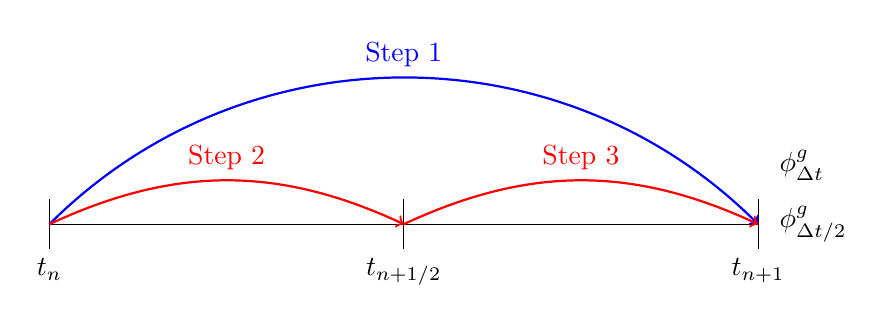
\begin{tikzpicture}[scale=1.5]
\draw[] (0,2) -- (6,2) ;
\foreach \x in  {0,3,6}
\draw[shift={(\x,2)},color=black] (0pt,6pt) -- (0pt,-6pt);
\draw[shift={(0,2)},color=black] (0pt,0pt) -- (0pt,-6pt) node[below] {$t_n$};
\draw[shift={(3,2)},color=black] (0pt,0pt) -- (0pt,-6pt) node[below] {$t_{n+1/2}$};
\draw[shift={(6,2)},color=black] (0pt,0pt) -- (0pt,-6pt) node[below] {$t_{n+1}$};
\draw (0,2) edge[out=45,in=135,->,thick,blue] node[above,sloped] {\tcb{Step 1}} (6,2);
\draw (0,2) edge[out=25,in=155,->,thick,red] node[above,sloped] {\tcr{Step 2}} (3,2);
\draw (3,2) edge[out=25,in=155,->,thick,red] node[above,sloped] {\tcr{Step 3}} (6,2);
\node[anchor=west](shape) at (6.1,2.5) {$\tcb{\phi_{\Delta t}^g}$};
\node[anchor=west](shape) at (6.1,2) {$\tcr{\phi_{\Delta t/2}^g}$};

\end{tikzpicture}
\caption{Visualization of step doubling process on time-line}
\label{fig:dt2_1}
\end{figure}

\begin{figure}[!htpb]
\centering
\begin{tikzpicture}[every node/.style = {font=\large},scale=0.75]

\node[blueblock](p1) at (-6,3) {Step 1} ;
\node[redblock](p2) at (-8,0) {Step 2} ;
\node[redblock](p3) at (-4,0) {Step 3} ;
\node[purpleblock](p4) at (0,0) {Compute \\ $e_n$};
\node[purpleblock](p5) at (4,0) {Compute  \\ $\Delta t_{new}$};
\node[greendiamond](p6) at (8,0) {$e_n < e_{tol}$};
\node[orangeblock](p7) at (0,-3) {Restore \\ Solutions};

\draw[->,thick](p1.east) -| (p4.north);
\draw[->,thick](p2.east) -- (p3.west);
\draw[->,thick](p3.east) -- (p4.west);
\draw[->,thick](p4.east) -- (p5.west);
\draw[->,thick](p5.east) -- (p6.west);
\draw[->,thick](p6.south) |- node[right] {no} (p7.east);
\draw[->,thick](p6.east) -- node[above] {yes} (11,0);
\draw[->,thick](p7.west) -| (-10,0) -- (p2.west);
\draw[->,thick](p7.west) -| (-10,0) |- (p1.west);

\end{tikzpicture}
\caption{Visualization of step doubling process with coding logic}
\label{fig:dt2_2}
\end{figure}

%%%%%%%%%%%%%%%%%%%%%%%%%%%%%%%%%%%%%%%%%%%%%%%%
\section{Delayed Neutron Precursor Updates}
\label{sect:dnp}
%%%%%%%%%%%%%%%%%%%%%%%%%%%%%%%%%%%%%%%%%%%%%%%%

This section presents the time-integration method used to solve coupled flux/shape and precursor equations, represented by Equations~\eqref{eq:flux}/\eqref{eq:shape}~and~\eqref{eq:precursor}/\eqref{eq:prec}. First, we note that we could keep this system of two time-dependent equations and solve it as a coupled system. However, this is unnecessary and a memory expensive endeavor because the precursor equation is only an ODE and not a PDE. Instead, one may discretize in time the shape equation, which typically requires the knowledge of the precursor concentrations at the end of the time step. This precursor value is taken from the solution, numerical or analytical, of the precursors ODE.

%%%%%%%%%%%%%%%%%%%%%%%%%%%%%%%%%%%%%%%%%%%%%%%%
\subsection{Precursor Evaluation Using Theta Method Time Discretization}

A common precursor evaluation technique is using the theta method, described in \sct{sect:theta}. Applying this to \eqt{eq:prec}:
\be
\frac{C^{n+1}-C^n}{\Delta t}=(1-\theta)\beta S_f^np^n-(1-\theta)\lambda C^n + \theta\beta S_f^{n+1}p^{n+1}-\theta\lambda C^{n+1}
\ee
Where $S_f$ is the fission source equivalent for shape ($S_f^n=(\nu\Sigma_f)^n\varphi^n$). Rearranging to solve for the precursor at the end of the time step yields
\be
C^{n+1} = \frac{1-(1-\theta)\Delta t\lambda}{1+\theta\Delta t\lambda}C^n + \frac{(1-\theta)\Delta t \beta}{1+\theta\Delta t\lambda}S_f^n p^n +  \frac{\theta\Delta t \beta}{1+\theta\Delta t\lambda}S_f^{n+1} p^{n+1}
\ee
Reporting this value of $C^{n+1}$, one can solve for the shape $\varphi^{n+1}$ as a function of $\varphi^n$ and $C^n$ (and $p^n$, $p^{n+1}$, $dp/dt|_n$ and  $dp/dt|_{n+1}$).
Once $\varphi^{n+1}$ has been determined, $C^{n+1}$ is updated.  Applying this technique to implicit discretization is done by changing the definition the fission source ($S_f^n=(\nu\Sigma_f)^n\varphi^n$) and eliminating all $p$ terms.

%%%%%%%%%%%%%%%%%%%%%%%%%%%%%%%%%%%%%%%%%%%%%%%%
\subsection{Analytical Precursor Integration}

Another technique to evaluating the precursor equation is to use a exponential operator and integrate the time derivative analytically.  Applying this operation to \eqt{eq:prec} yields:
\be
C^{n+1} =  C^n e^{-\lambda (t_{n+1} - t_n) }  + \int_{t_n}^{t_{n+1}} \beta(t') S_f(t') p(t')e^{-\lambda (t_{n+1}-t')}dt'
\label{eq:prec_an}
\ee
Again, this can be applied to implicit discretization by altering the definition of the fission source and eliminating $p$.  Because $S_f$ is not known continuously over the time step, the integration can be done using any schemet (Riemann, trapezoid, Simpson's, etc.). However, there is a very accurate representation of $p(t)$ over the macro step from the PRKE solve. In order to utilize this information, another possibility is to interpolate $S_f$ linearly over the macro step.  Such that:
\be
S_f(t) = \frac{t_{n+1}-t}{t_{n+1}-t_n}S_f^n  + \frac{t-t_n}{t_{n+1}-t_n}S_f^{n+1}  \quad t_n \le t \le t_{n+1}
\ee
Applying this to \eqt{eq:prec_an} yields:
\be
C^{n+1} = C^n e^{-\lambda \Delta t} + \left(\hat{a}_2 S_f^{n+1}+\hat{a}_1 S_f^n\right)\beta
\ee
With integration coefficients defined as:
\begin{align}
&\hat{a}_1= \int_{t_n}^{t_{n+1}}\frac{t_{n+1}-t'}{\Delta t}p(t')e^{-\lambda(t_{n+1}-t')}dt' \\
&\hat{a}_2 = \int_{t_n}^{t_{n+1}}\frac{t'-t_n}{\Delta t}p(t')e^{-\lambda(t_{n+1}-t')}dt'
\end{align}
The amplitude $(p)$ is included in the integration coefficient because it has been highly accurately calculated in the micro step scheme, so a piecewise interpolation (linear, cubic, etc.) between those points can be done to maximize accuracy.



%%%%%%%%%%%%%%%%%%%%%%%%%%%%%%%%%%%%%%%%%%%%%%%%
%%%%%%%%%%%%%%%%%%%%%%%%%%%%%%%%%%%%%%%%%%%%%%%%
\section{Rattlesnake Implementation}
%%%%%%%%%%%%%%%%%%%%%%%%%%%%%%%%%%%%%%%%%%%%%%%%
%%%%%%%%%%%%%%%%%%%%%%%%%%%%%%%%%%%%%%%%%%%%%%%%

Rattlesnake is a MOOSE-based application developed INL specific to solving radiation transport problems with multiphysics capabilities.  MOOSE is a finite-element based, multiphysics framework that gives the general architecture for the development of physics application like Rattlesnake.   At the heart of Rattlesnake is the action system, which provides a means to consolidate the MOOSE input syntax (which can be quite larger for multigroup transport simulations), so that a user does not have to define every kernel, variable, etc., used in the problem. Rather, the user inputs an equation description 
(e.g., Diffusion, S$_n$, P$_n$, etc.) and a solution method (e.g., SAAF, LS, CFEM, DFEM, etc.), and the action system will incorporate all the necessary physics involved (kernels, boundary conditions, postprocessor, etc.).

 
%%%%%%%%%%%%%%%%%%%%%%%%%%%%%%%%%%%%%%%%%%%%%%%%
\subsection{Executioner}
%%%%%%%%%%%%%%%%%%%%%%%%%%%%%%%%%%%%%%%%%%%%%%%%

An IQS excecutioner was created to implement the IQS method. The IQS executioner derives from the Transient executioner in MOOSE.  The IQS executioner contains a loop over micro time steps that computes the PRKE solution and then passes $p$ and $\frac{dp}{dt}$ for the Transient executioner to evaluate the shape equation at each macro step.  The PRKE solve is performed with a user specified option of backward-Euler, Crank-Nicholson, or SDIRK33.   The IQS executioner also supplements Transient Picard iteration process by adding its own error criteria:
\be
Error_{IQS}=\left|\frac{\sum_{g=1}^G\left(\phi^{*g},\frac{1}{v^g}\varphi^{g,n}\right)}{\sum_{g=1}^G\left(\phi^{*g},\frac{1}{v^g}\varphi^{g,0}\right)}-1\right|
\label{eq:eiqs}
\ee

%%%%%%%%%%%%%%%%%%%%%%%%%%%%%%%%%%%%%%%%%%%%%%%%
\subsection{Action System}
%%%%%%%%%%%%%%%%%%%%%%%%%%%%%%%%%%%%%%%%%%%%%%%%

The IQS implementation mostly require the specific IQS executioner, described above. However, IQS additional changes are in the Rattlesnake action system in order to support the IQS execution.  First, changes needed to be made in order to evaluate the shape equation.  The shape equation, after some manipulation, is very similar to the time-dependent governing laws that Rattlesnake already solves. Using multigroup diffusion as an example again, we show the various kernels employed and highlight the new or modified kernels.

\begin{align}
\frac{\partial}{\partial t}\left(\frac{\varphi^g}{v^g}\right)=&\underbrace{\frac{\chi_p^g}{\keff} \sum_{g'=1}^G (1-\beta) \nu^{g'} \Sigma_f^{g'} \varphi^{g'}}_{Flux Kernel} + \underbrace{\sum_{g'\neq g}^G\Sigma_s^{g'\to g} \varphi^{g'}}_{Flux Kernel} - \underbrace{\left( -\div D^g \grad \right)\varphi^g}_{Flux Kernel} - \underbrace{\Sigma_r^g\varphi^g}_{Flux Kernel} \nonumber \\
& - \underbrace{\frac{1}{v^g} \boxed{\overbrace{\frac{1}{p}\frac{dp}{dt}}^{From Executioner}}\varphi^g}_{IQS Kernel}+\underbrace{\frac{1}{p}\sum_{i=1}^I\chi_{d,i}^g\lambda_iC_i}_{Modified Flux Kernel}
\end{align}

To enable Rattlesnake to solve this equation, an IQS removal kernel was created to evaluate $\sum_{g=1}^G\frac{1}{v^g}\frac{1}{p}\frac{dp}{dt}\varphi^g$ and added when the IQS executioner is called.  Also, the precursor kernel was modified to include the $\frac{1}{p}$ term. Finally, the precursor auxkernel that evaluates \eqt{eq:prec} using the analytical integration method described in \sct{sect:dnp}.

%%%%%%%%%%%%%%%%%%%%%%%%%%%%%%%%%%%%%%%%%%%%%%%%
\subsection{PRKE coefficients}
%%%%%%%%%%%%%%%%%%%%%%%%%%%%%%%%%%%%%%%%%%%%%%%%

In order to evaluate the PRKE coefficients, defined by Equations~\ref{eq:rmb}~-~\ref{eq:l}, four postprocessors were created.  The parameter calculations were separated by $\frac{\bar{\beta}_i}{\Lambda}$ numerator, $\bar{\lambda}_i$ numerator/denominator, $\frac{\rho-\bar{\beta}}{\Lambda}/\frac{\bar{\beta}}{\Lambda}$ denominator, and $\frac{\rho-\bar{\beta}}{\Lambda}$ numerator. The first three are relatively simple, only relying on material properties and solution quantities, then computing the elemental integral.  The $\frac{\rho-\bar{\beta}}{\Lambda}$ numerator requires the use of the MOOSE \texttt{save\_in} feature. This feature saves the residual from a calculated kernel or boundary contribution in the shape evaluation to an auxiliary variable.  The postprocessor then computes the inner product of this variable and the initial adjoint solution.  After each of these postprocessors are evaluated, a user object pulls together all the values and performs the numerator/denominator divisions.  The resulting values are then passed to the executioner for the PRKE solve.

%%%%%%%%%%%%%%%%%%%%%%%%%%%%%%%%%%%%%%%%%%%%%%%%
\subsection{Other Action Systems}
%%%%%%%%%%%%%%%%%%%%%%%%%%%%%%%%%%%%%%%%%%%%%%%%

For simplicity, IQS implementation has only been described for CFEM diffusion.  However, Rattlesnake has other action systems capable of transient simulation, where IQS can be implemented and be effective.  One of these action systems is DFEM diffusion, where the only major difference from CFEM is the diffusion term in Equations~\eqref{eq:flux}~and~\eqref{eq:shape}.  However, in the derivation for IQS, this term is unaffected between shape and flux evaluation.  So saving the residual for this diffusion kernel in the \texttt{save\_in} variable is the only alteration to this action for IQS to function.\\
Additional action systems involve transport, but it is evident from \sct{sect:transport} that IQS implementation in these is straightforward as well.  The main differences between a diffusion implementation and a transport implementation are outlined below:
\begin{enumerate}
\item The form of the operators in the shape equations is different, but Rattlesnake has already implemented all the kernels necessary to represent these operators.  So no change is necessary to these kernels is necessary for IQS.  Additionally, the $\frac{1}{v^g}\frac{1}{p}\frac{dp}{dt}$ is the same, so both action systems can use the same kernel.
\item The PRKE parameters also change because of the operators.  For the $(\rho-\bar{\beta})$ parameter, the same post-processor can be used with the \texttt{save\_in} functionality in MOOSE.  The post-processor for $\bar{\beta}_i$ must be re-written for transport, but takes a very similar form as diffusion.
\end{enumerate}

IQS will be made available to any action system capable of transient simulation, which includes:
\begin{itemize}
\item CFEM-Diffusion
\item DFEM-Diffusion
\item SAAF-CFEM-SN
\item SAAF-CFEM-PN
\item LS-CFEM-SN
\item DFEM-SN
\end{itemize}

%%%%%%%%%%%%%%%%%%%%%%%%%%%%%%%%%%%%%%%%%%%%%%%%
\subsection{Predictor-Corrector Modification}
%%%%%%%%%%%%%%%%%%%%%%%%%%%%%%%%%%%%%%%%%%%%%%%%

In order to preserve the already implemented standard version of IQS, an option in the IQS executioner was created to specify which method is desired.  Because the diffusion solve is flux instead of shape, when predictor-corrector option is specified, the IQS removal kernel ($\frac{1}{v^g}\frac{1}{p}\frac{dp}{dt}$) and the modified precursor kernel are bypassed, while all the postprocessors are still executed.  However, it is difficult to rescale the flux to shape before the PRKE parameter postprocessor are executed.  So the parameters are computed using the full flux, but amplitude is space independent and comes out of the integrals.  As seen in parameter definitions, when shape is replaced with flux, the amplitude comes out of the integral and cancels out.  So the conversion of the predicted flux in  \eqt{eq:rescale} to shape is unnecessary if the corrected flux is solved with \eqt{eq:phicorr2}.  After obtaining the corrected flux, the precursors are re-evaluated using a \texttt{EXEC\_LINEAR} statement.
\be
\underbrace{\phi^g_{n+1}}_{\text{corrected}} = \underbrace{\phi^g_{n+1}}_{\text{predicted}} \frac{K_0}{K_{n+1}} p_{n+1}
\label{eq:phicorr2}
\ee

%%%%%%%%%%%%%%%%%%%%%%%%%%%%%%%%%%%%%%%%%%%%%%%%
\subsection{Input}
%%%%%%%%%%%%%%%%%%%%%%%%%%%%%%%%%%%%%%%%%%%%%%%%

The input file for IQS is very similar to the current transient diffusion input file.  The IQS input has a different executioner type and parameters.  The executioner type is simply IQS and input parameters include the number of micro time steps per macro step, the IQS error tolerance, and the initial power.  The Rattlesnake transient action system currently requires a multi-app and transfer to compute and pass the initial $\phi$ and $\keff$, which is present in the transient input deck.  However, IQS also requires an initial evaluation of the adjoint flux, for the weighting function.  So another input file and multi-app transfer was made for the adjoint calculation.  \vspace{3mm}

Below is the syntax for the executioner block for an IQS input file.  The \texttt{predictor\_corrector} logical determines whether to do IQS P-C or regular IQS.  The \texttt{IQS\_error\_tol} is the tolerance for the IQS error represented by \eqt{eq:eiqs} and will at most \texttt{picard\_max\_its} iterations until convergence.  The \texttt{prke\_scheme} defines the time discretization used for the PRKE solution. Where \texttt{RK} is SDIRK33, \texttt{CN} is Crank-Nicholson, and \texttt{IE} is implicit-Euler.
\begin{lstlisting}
[Executioner]
  type = IQS
  predictor_corrector = true/false
  picard_max_its = 5
  ...
  n_micro = 10000
  IQS_error_tol = 1e-7
  prke_scheme = 'RK'
[]
\end{lstlisting}

Since IQS needs to use the adjoint solution for the PRKE parameter evaluation, auxiliary variables need to be created for each group in the input file.  Below is an example of their definition: 
\begin{lstlisting}
[AuxVariables]
  [./adjoint_flux_g0] 
    family = LAGRANGE
    order = FIRST
  [../]
  [./adjoint_flux_g1]
    family = LAGRANGE
    order = FIRST
  [../]
  ...
[]
\end{lstlisting}

Below is the syntax for the multi-app block to perform forward and adjoint steady-state evaluations:
\begin{lstlisting}
[MultiApps]
 [./initial_solve]
   type = FullSolveMultiApp
   execute_on = initial
   input_files = initial.i
 [../]
 [./adjoint_solve]
   type = FullSolveMultiApp
   execute_on = initial
   input_files = adjoint.i
 [../]
[]
\end{lstlisting}

Below is the syntax for the Transfer block to copy the initial and adjoint solutions from the multi-apps.
\begin{lstlisting}
[Transfers]
 [./copy_solution]
   type = TransportSystemVariableTransfer
   direction = from_multiapp
   multi_app = initial_solve
   execute_on = initial
   from_transport_system = diff
   to_transport_system = diff
 [../]
 [./copy_adjoint]
   type = MultiAppVariableTransfer
   execute_on = initial
   direction = from_multiapp
   multi_app = adjoint_solve
   from_variables = 'sflux_g0 sflux_g1 ...'
   to_variables = 'adjoint_flux_g0 adjoint_flux_g1 ...'
 [../]
 [./copy_eigenvalue]
   type = EigenvalueTransfer
   execute_on = initial
   direction = from_multiapp
   multi_app = initial_solve
 [../]
[]
\end{lstlisting}


